\section{Data Analysis}
Data analysis is the act of analyzing, cleansing, manipulating, and modeling data in order to identify usable information, generate conclusions, and help decision-makings~\cite{Book:sbrown_2014_transforming}.
Data analysis has several dimensions and approaches, including a wide range of techniques known by various names and applied in a variety of business, science, and social science sectors~\cite{Book:pruneau_2017}.

In today's corporate world, data analysis plays an important part in making decisions more scientific and assisting firms in operating more efficiently.
\ac{DM} is a type of data analysis technique that focuses on statistical modeling and knowledge discovery for predictive rather than purely descriptive purposes,
whereas \ac{BI} is a type of data analysis that focuses on aggregation and is primarily concerned with business information, more on this later.

Furthermore, Data analysis, in statistical applications, can be separated into descriptive statistics, \ac{EDA}, and \ac{CDA}~\cite{Book:doing_data_science}. 
\ac{EDA} is concerned with finding new features in data, whereas \ac{CDA} is concerned with validating or refuting current assumptions.[citation?] 
Predictive analytics focuses on the application of statistical models for predictive forecasting or classification, 
while text analytics, applies statistical, linguistic, and structural techniques to extract and classify information from textual sources, a species of unstructured data.
All of the aforementioned are examples of data analysis~\cite{Article:goodnight_2011_the}.

\subsection{Procedure for analyzing data}
\begin{figure}[t]
    \centering
    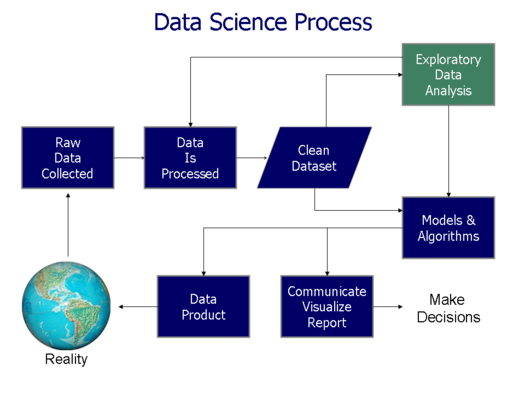
\includegraphics[width=0.9\textwidth]{content/chapter_1/images/Data_visualization_process_v1.png}
    \caption{Data science process flowchart (Source:~\cite{Book:doing_data_science})}
    \label{fig:data-science-flowchart}
\end{figure}
The term \textit{``analysis''} refers to the process of breaking down a whole into its constituent parts for closer evaluation.
Data analysis is the act of getting raw data and then transforming it into information that users can utilize to make decisions~\cite{Book:sbrown_2014_transforming}.
Data is gathered and processed in order to answer questions, test hypotheses, or refute theories[].
Statistician \citeauthor{Article:future_of_data_tukey}, defined data analysis in 1961, as:
\begin{quote}
    ``Procedures for analyzing data, techniques for interpreting the results of such procedures, ways of planning the gathering of data to make its analysis easier, 
    more precise or more accurate, and all the machinery and results of (mathematical) statistics which apply to analyzing data.''~\cite{Article:future_of_data_tukey}
\end{quote}
There are various distinct phases that can be identified as show in \ref{fig:data-science-flowchart}, these are iterative in the sense that input from later phases may lead to further effort in earlier ones~\cite{Book:doing_data_science}.
Similar stages can be found in the \ac{CRISP} framework, which is used in \acl{DM}.

% \paragraph{Connection to the Scientific Method}
\subsubsection{Connection to the Scientific Method}
We can think of the data science process as an extension of or variation of the scientific method:
\begin{itemize}
    \item Ask a question.
    \item Do background research.
    \item Construct a hypothesis.
    \item Test your hypothesis by doing an experiment.
    \item Analyze your data and draw a conclusion.
    \item Communicate your results.
\end{itemize}
In both the data science process and the scientific method, not every problem requires one to go through all the steps, but almost all problems can be solved with \textit{some} combination of the stages~\cite{Book:doing_data_science}.
For example, if your end goal is a \textbf{data visualization} (which itself could be thought of as a data product), it’s possible you might not do any machine learning or statistical modeling,
but you would want to get all the way to a clean dataset, do some \acl{EDA}, and then create the visualization. This has happened to me many times during my internship, as we will see in [Chapter 4].

\subsection{What is Data?}
We talked a lot about data in the last subsection and while it is important that we can analyze and understand data, 
Understanding what data is is a prerequisite for being able to use it properly, and it is perhaps the most important thing in my professional judgement.
Data is no longer only a collection of numbers and classified variables.
A strong data scientist needs to be versatile and comfortable with dealing a variety of types of data, including:
\begin{itemize}
    \item Traditional: numerical, categorical, or binary
    \item Text: emails, tweets, New York Times articles
    \item Records: user-level data, timestamped event data, log files
    \item Complex: Geo-based location data (GIS), Network \& Images
    \item Sensor data, my case (see Chapter [])
\end{itemize}

% On how to deal with different types of data, it represents open research questions for the statistical and computer science community. 
% This is the frontier! Since some of these are open research problems, in practice, data scientists do the best they can, and often invent new methods as part of their work.

\subsection{Data Cleaning}
\subsection{Data Transformation}
\subsection{Data Reduction}